\documentclass{standalone}

%--------------------------------------------------------------------------------------------------------
% PAQUETES
%--------------------------------------------------------------------------------------------------------

\usepackage{tikz}
\usepackage{tkz-euclide}
\usepackage{siunitx}
\usepackage{fourier}

%--------------------------------------------------------------------------------------------------------
% OTRAS CONFIGURACIONES
%--------------------------------------------------------------------------------------------------------

\usetkzobj{all}

%--------------------------------------------------------------------------------------------------------
% INICIO DEL DOCUMENTO
%--------------------------------------------------------------------------------------------------------

\begin{document}
	
	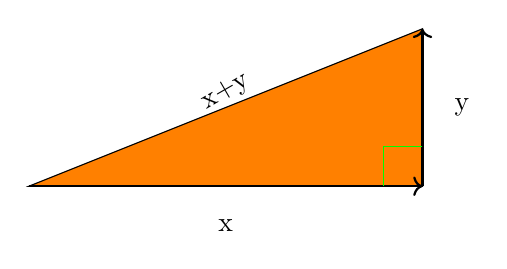
\begin{tikzpicture}
		%\draw[blue] (-5,0) grid (2,4);
		%\draw[red] (0,0) circle (1mm);
		
		\draw [fill=orange](1,1) --(-4,1) -- (1,3) -- cycle;
		\draw [thick,<-](1,1) --(-4,1);
		\draw [thick,->](1,1) -- (1,3);
		\draw [green] (1,1.5) -- (0.5,1.5) -- (0.5,1);

		\node at (-1.5,0.5) {x};
		\node at (1.5,2) {y};
		\node [ rotate=30] at (-1.5,2.2) {x+y};
		
	\end{tikzpicture}

\end{document}